% Copyright 2004 by Till Tantau <tantau@users.sourceforge.net>.
%
% In principle, this file can be redistributed and/or modified under
% the terms of the GNU Public License, version 2.
%
% However, this file is supposed to be a template to be modified
% for your own needs. For this reason, if you use this file as a
% template and not specifically distribute it as part of a another
% package/program, I grant the extra permission to freely copy and
% modify this file as you see fit and even to delete this copyright
% notice. 

\documentclass{beamer}
\usepackage{graphicx}
\usepackage{breqn}
\graphicspath{ {images/} }
\usepackage{amsmath}
\usepackage{dsfont}
% There are many different themes available for Beamer. A comprehensive
% list with examples is given here:
% http://deic.uab.es/~iblanes/beamer_gallery/index_by_theme.html
% You can uncomment the themes below if you would like to use a different
% one:
%\usetheme{AnnArbor}
%\usetheme{Antibes}
%\usetheme{Bergen}
%\usetheme{Berkeley}
\usetheme{Berlin}
%\usetheme{Boadilla}
%\usetheme{boxes}
%\usetheme{CambridgeUS}
%\usetheme{Copenhagen}
%\usetheme{Darmstadt}
%\usetheme{default}
%\usetheme{Frankfurt}
%\usetheme{Goettingen}
%\usetheme{Hannover}
%\usetheme{Ilmenau}
%\usetheme{JuanLesPins}
%\usetheme{Luebeck}
%\usetheme{Madrid}
%\usetheme{Malmoe}
%\usetheme{Marburg}
%\usetheme{Montpellier}
%\usetheme{PaloAlto}
%\usetheme{Pittsburgh}
%\usetheme{Rochester}
%\usetheme{Singapore}
%\usetheme{Szeged}
%\usetheme{Warsaw}

\title{Effects of Unemployment Benefits and Uncertainty in Heterogeneous Models}

% A subtitle is optional and this may be deleted
\subtitle{}

\author{Eric, Yannic and Andrian}
% - Give the names in the same order as the appear in the paper.
% - Use the \inst{?} command only if the authors have different
%   affiliation.

%\institute[Universities of Somewhere and Elsewhere] % (optional, but mostly needed)
%{
% \inst{1}%
%  Department of Computer Science\\
%  University of Somewhere
%  \and
%  \inst{2}%
%  Department of Theoretical Philosophy\\
%  University of Elsewhere}
% - Use the \inst command only if there are several affiliations.
% - Keep it simple, no one is interested in your street address.

%\date{Conference Name, 2013}
% - Either use conference name or its abbreviation.
% - Not really informative to the audience, more for people (including
%   yourself) who are reading the slides online

%\subject{Theoretical Computer Science}
% This is only inserted into the PDF information catalog. Can be left
% out. 

% If you have a file called "university-logo-filename.xxx", where xxx
% is a graphic format that can be processed by latex or pdflatex,
% resp., then you can add a logo as follows:

% \pgfdeclareimage[height=0.5cm]{university-logo}{university-logo-filename}
% \logo{\pgfuseimage{university-logo}}

% Delete this, if you do not want the table of contents to pop up at
% the beginning of each subsection:
\AtBeginSubsection[]
{
  \begin{frame}<beamer>{Outline}
    \tableofcontents[currentsection,currentsubsection]
  \end{frame}
}


% Let's get started
\begin{document}



\begin{frame}
  \titlepage
\end{frame}

\begin{frame}{Outline}
  \tableofcontents
  % You might wish to add the option [pausesections]
\end{frame}

% Section and subsections will appear in the presentation overview
% and table of contents.
\section{Introduction}
\subsection{}
\begin{frame}{The complete market framework}
  \begin{itemize}

  \item {
  Results
  }
	\begin{enumerate}
		\item{
		Outcomes are efficient - there is no alternative in which all households can be made better off.
		}
		\item{
		These models do not produce any inequality in well-being for identical households starting from identical positions. 
		}
	\end{enumerate}
		
  \item {
  Limitations  
  }
	\begin{enumerate}
		\item{
Unrealistic assumption of full insurance.
		}
		\item{
Limitation in questions we can ask. Impossible to ask questions, where differences across people might affect macroeconomic outcomes.
		}
	\end{enumerate}

  \end{itemize}

\end{frame}

\begin{frame}{Heterogeneity in models}
  \begin{itemize}

  \item {
  Uninsured risk
  }
	\begin{enumerate}
		\item{
Introduction of idiosyncratic or uncorrelated risk among individuals.
		}
		\item{
Accompanied by incomplete markets.
		}
		\item{
In such an environment aggregate risk may create further differences across groups of people.
		}
	\end{enumerate}
		
\item{
Differences among decisionmakers.
}

  \end{itemize}
\end{frame}

\begin{frame}{Why these models?}
	\begin{itemize}
	
	\item {
	Why the Aiyagari Model? 
	}
	\begin{enumerate}
	\item {
Allows for the study of agents' savings behavior while facing idiosyncratic risk in an incomplete market framework, where only part of the risk is covered by, for instance, public institutions. 
	}
	\item {
How does the bahvior of selfinsured agents change when public insurance systems, such as UI, change? 
	}
	\item {
	How do these changes in behavior in turn affect the other economic variables?
	}
	\item {	
	When would agents prefer a change and when not? Do these changes affect different groups differently? 
	}	
	\end{enumerate}

	\end{itemize}

\end{frame}

\begin{frame}{Why these models?}
	\begin{itemize}
	
	\item {
	Why the Krussell Smith model? 
	}
	
	\begin{enumerate}
	
	\item {
Aggregate shocks might affect different groups in a contrasting manner.  
	}
	\item {
Helps to improve redistributional policy measures in business cycles.
	}

	\end{enumerate}

	\end{itemize}

\end{frame}


\section{The Aiyagari Model}
\subsection{Model Setup}

\begin{frame}{Why these models?}
	\begin{itemize}
	
	\item {
	Consumers 
	}
	

	\end{itemize}

\end{frame}




\subsection{Mechanics governing the model}


\section{Aggregate Uncertainty}
\subsection{}

\begin{frame}{Idiosyncratic Uncertainty}
	\begin{itemize}
	
	\item {
	Why the Aiyagari Model? - Explaining the 				differences from the Representative Agent Model.
	}
	\item {
	Model Mechanics - How does a change in 					idiosyncratic uncertainty affect the agents' behavior?
	}
	\item {
	What conclusions can we draw from such an analysis?
	}
	\item {
	Where are the model's limitations?
	}		
	\end{itemize}
	  \centering{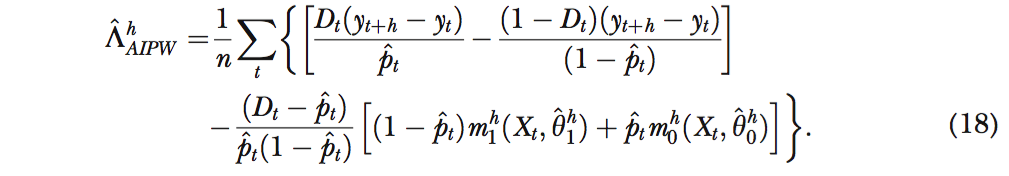
\includegraphics[scale=0.30]{eq18}}

\end{frame}


\end{document}